% ==================================================
\chapter{Software Design}\label{chap:Software Design}
% ==================================================

% --------------------------
\section{Data Sources}
% --------------------------
There were several options to get bibliographic data for powering the publication plot of Scholar Plot (SP). These include \href{http://www.scopus.com/}{Scopus}, \href{http://www.isiknowledge.com/}{ISI Web of Knowledge}, and \href{http://scholar.google.com}{Google Scholar}. We chose Google Scholar for two reasons: a) it is all inclusive, covering all types of publications such as journals, conferences, books, and patents; and, b) it is freely available. Scopus is subscription based and not as inclusive as Google Scholar. ORCID has publications and funding data but requires extensive set-up.

Our choice carries a few challenges, too. Google Scholar does not provide an application programming interface. Hence, we had to develop an elaborate software to scrape information off publicly available Google Scholar pages. Also, not every academic has a Google Scholar page. %This has been changing fast, however, as one college started to maintain a Google Scholar page after the other in the United States mandating their faculty to maintain a Google Scholar page.

We use the Journal IF List that is issued every year by Thompson Reuters to assign disk sizes to journal publications.

For funding records, we use the publicly available grant records from the National Science Foundation (NSF) \cite{nsf}, the National Institutes of Health (NIH) \cite{nih}, and the National Aeronautics and Space Administration (NASA) \cite{nasa}. These are the only funding agencies with publicly available datasets at this point.

\begin{table}[h!]
\centering
\begin{tabular}{||c c c c||}
 \hline
 Agencies & Fiscal Year & Rows & Per Year \\ [1ex]
 \hline\hline
 NSF & FY 1985 - FY 2013 & 312,311 rows & 10,769/year \\
 NIH & FY 2000 - FY 2013 & 777,657 rows & 55,456/year \\
 NASA & FY 2007 - FY 2015 & 16,670 rows & 1,852/year \\ [1ex]
 \hline
\end{tabular}
\caption{Funding datasets in Scholar Plot system.}
\label{table:1}
\end{table}









% --------------------------
\section{System Architecture}
% --------------------------


Scholar Plot is the web-based data visualization method that uses HTML5, CSS3, and SVG to render a scholar's accomplishment at a glance. We created a MySQL database to store the mapping between the scholar names and their Google Scholar IDs. We also designed and created database tables for NSF/NIH/NASA funding data. The user can search the name of the scholar in a text field. When the user starts to enter the name of the scholar, the names in our database which are similar to the entered name will be listed as a drop down list. We use jQuery and Ajax (asynchronous JavaScript and XML) method to have this feature, which connects to the database to get the list of names. If there are no matching/similar names, the user can also insert her/his Google Scholar ID to the database by one click event.

\begin{figure}[H]
\centering
  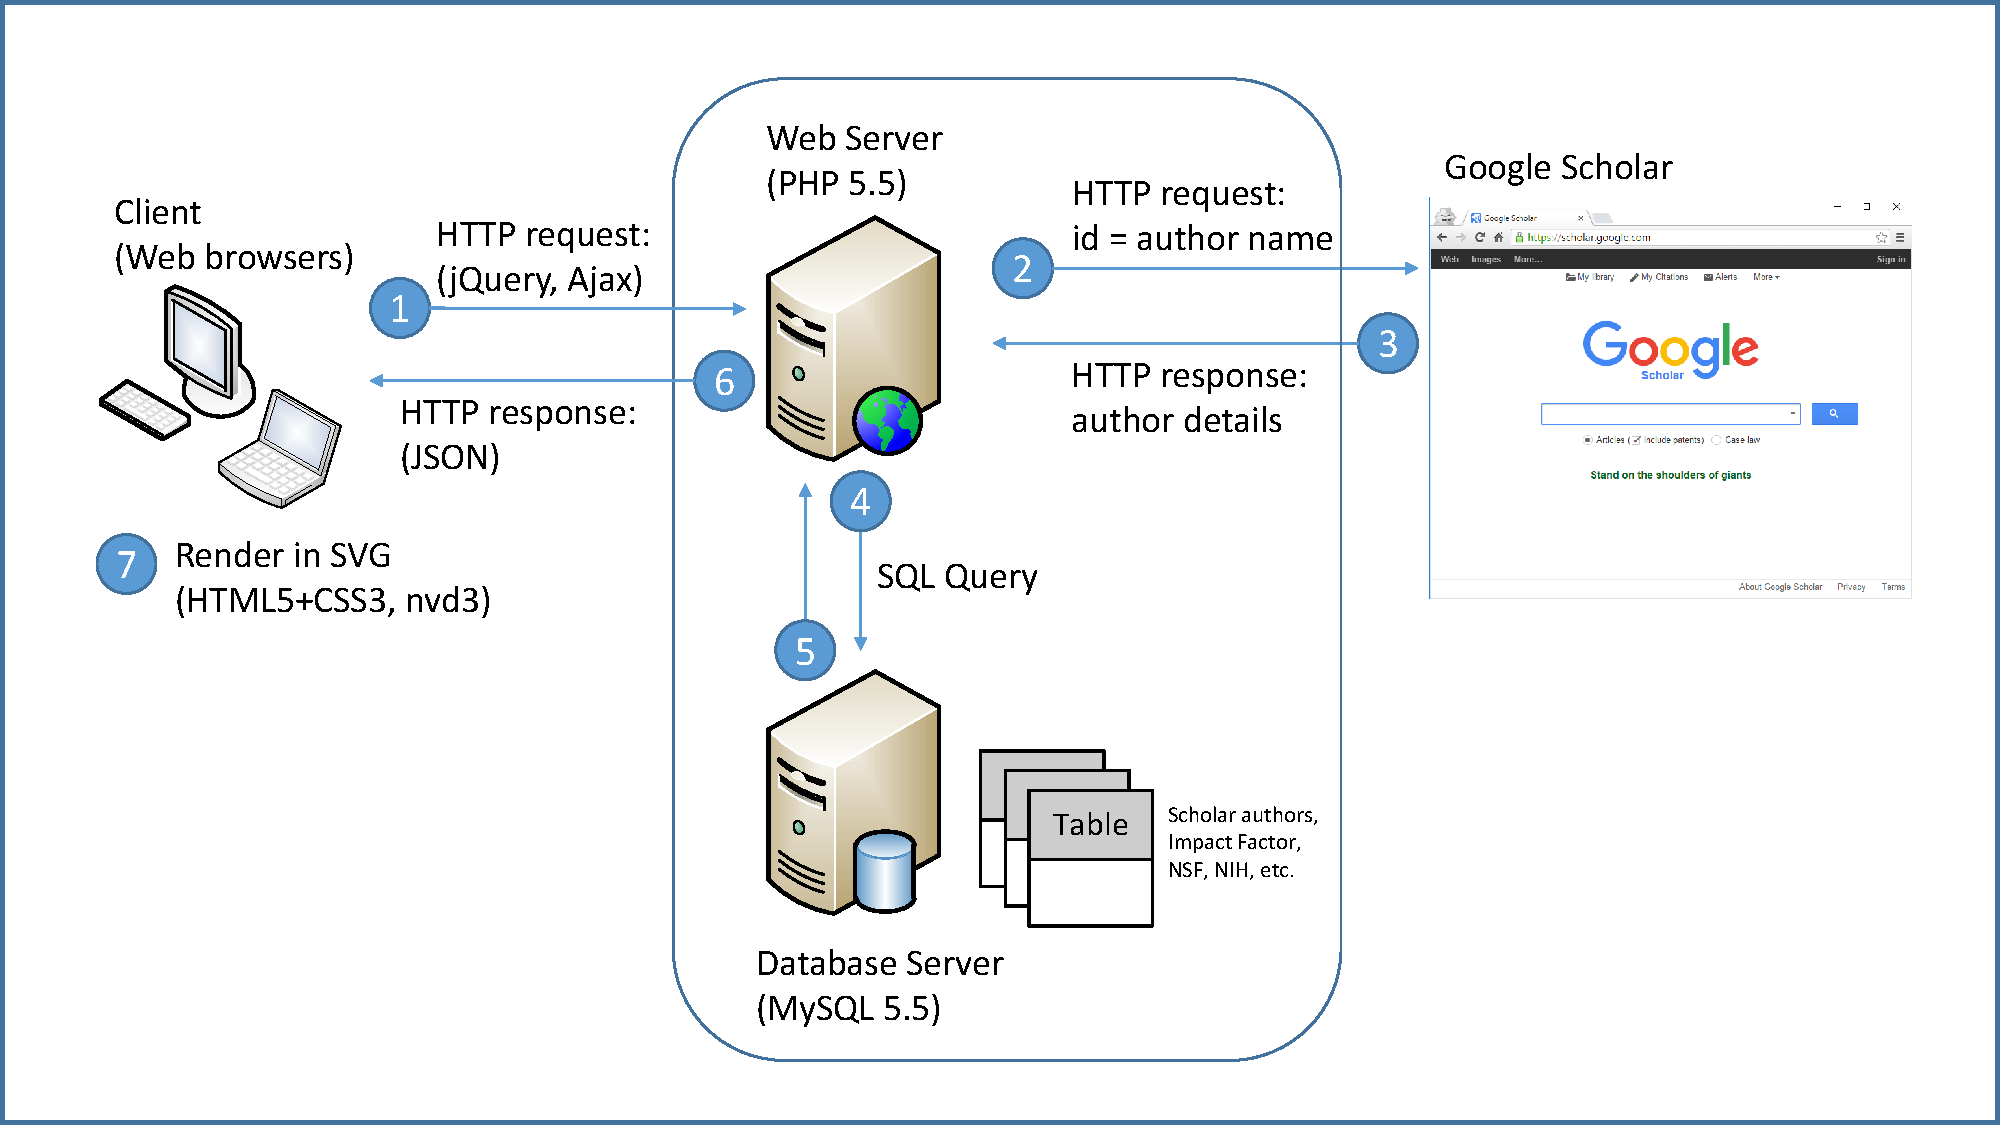
\includegraphics[width=1\textwidth]{figures/fig_system_architecture.pdf}
  \caption{System Architecture of Scholar Plot.}~\label{fig-arch}
%\vspace{-1ex}
\end{figure}

Once the scholar's name is selected, the user can run the application to see the visual results of the selected scholar's publications and fundings. Scholar Plot connects to the Web server to retrieve the necessary information.
The server-side application is implemented in PHP scripting language and MySQL. The HTTP protocol is used for communicating between client-side and server-side to get the basic information via JSON format (JavaScript Object Notation) and JSONP function (Figure \ref{fig-arch}). Scholar Plot also uses htmlSQL library to parse Google Scholar's page to extract user basic information \cite{htmlSQL}.

%, collecting for the publication title, the journal name, the co-authors' name, the year, and the citations. It also collects the {\it h-}index and the number of total citations from the top of the scholar's page up to 300 publications.

Scholar Plot obtains the Impact Factor ($IF$) for a particular journal from our database. The data of Impact Factor is acquired from The Thomson Reuters Impact Factor - Web of Science. Based on all this information it constructs the plots as per the design outlined in the Visualization and User Interface section, using nvd3 library \cite{nvd3org}.

The NSF/NIH/NASA funding datasets are available at the respective US government websites in various file formats such as XML, CSV, and so on \cite{nsf, nih, nasa}. We implemented a script to parse this massive XML dataset into our data structure that consists of AwardID, AwardAmount, First name, Last name, and Investigator by RoleCode (Principal Investigator, Co-Principal Investigator, and Former Principal Investigator), using XMLStarlet \cite{XMLStarlet}. We imported this data to our database using Toad DBMS tool. Currently, we have only these three funding data sources. So this is a limitation of the current system. It is biased to the scholar's country of residence. We are working on adding more of them to our database. %We designed our relational database schema in MySQL.




% ==================================================
% \chapter{Algorithms}\label{chap:Algorithms}
% ==================================================
% --------------------------
\section{Name Disambiguation}
% --------------------------


With the amount of data and data sources rapidly growing and expanding, it is essential for the large amounts of available data to be organized for analysis. Through the process known as Data Wrangling, unorganized and scattered data can be prepared for easy access and analysis. The datasets of google and goverment funding have to be cleaned because it contains many non-english characters and its messy datasets \cite{kang2008interactive}. We use regular expression to remove the invalid special characters and translate phonetic characters to English alphabets. We designed and implemented Algorithms \ref{algorithm} to match the author names in Google Scholar with those in NSF/NIH/NASA data. This process helps to improve the quality of results.


\subsection{Within the Google Scholar profile}

A single Google Scholar profile might contain multiple variations of the authors name based on the middle name and initials. For example, consider the example Google Scholar profile of Ioannis Pavlidis. It contains four variations of his name in different publications.

\begin{itemize}
\item Ioannis T Pavlids
\item IT Pavlids
\item I Pavlids
\item Ioannis Pavlids
\end{itemize}

We use the first initial and last name of an author to obtain the count of the number of publications in the panel.

\begin{figure}[H]
\begin{center}
  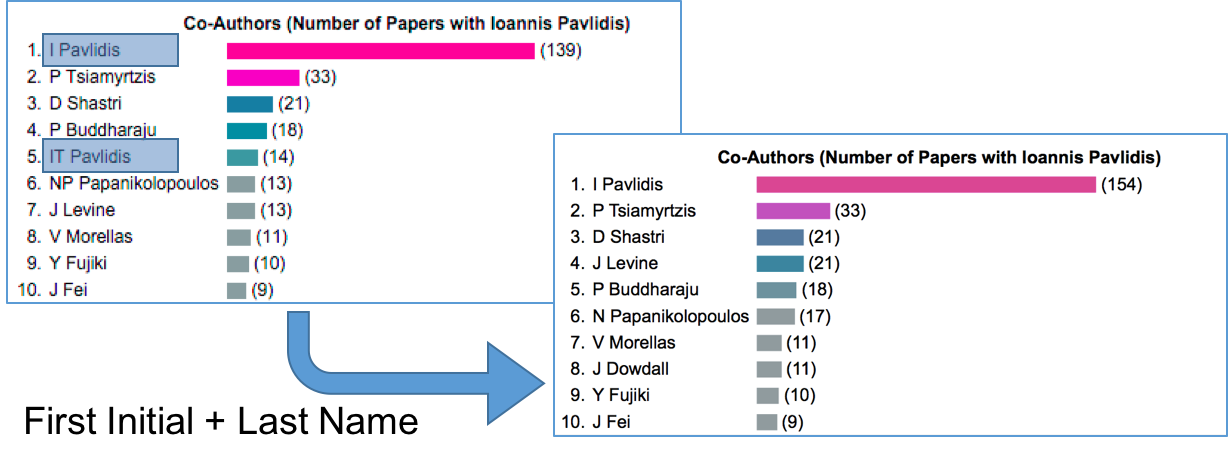
\includegraphics[width=.9\textwidth]{figures/fig-name-dis-example1}
\caption{Example of how the name disambiguation algorithm works.}
\label{default}
\end{center}
\end{figure}




% --------------------------
\subsection{Between Google Scholar and Funding datasets}
% --------------------------

The funding datasets released from governments need to be cleaned because they are different data formats and structure. We cleaned the names by removing Sr., Jr., III, Ph.D., Dr., and so on. Then we need to match the names in the Google Scholar profile with those in the funding datasets. The algorithm is given in Algorithm \ref{algorithm}. An example is visually depicted in Figure \ref{alg-example}.

\begin{figure}
\begin{algorithm}[H]
\caption{Matching the name between Google Scholar and funding datasets.}
\begin{algorithmic}[1]
\Procedure{Searching for Author Name}{}
\State $\textit{googleFirstName} \gets \text{first name in Google Scholar }$
\State $\textit{googleLastName} \gets \text{last name in Google Scholar }$
\State $\textit{googleMiddleInitial} \gets \text{middle initial in Google Scholar }$
\If {$lastNameInFundingData = googleLastName$}
\If {$firstNameInFundingData = googleFirstName$} 
\If {$googleMiddleInitial$ is null } 
{\Return true}
\Else{
\text{Search for} ($middleInitial, googleFirstName$) and ($googleFirstName, middleInitial$) 
\If { $found$} \Return true
\Else{ \Return false}
\EndIf
}
\EndIf
\EndIf
\EndIf
\Return false
\EndProcedure
\label{algorithm}
\end{algorithmic}
\end{algorithm}
\end{figure}



\begin{figure}[H]
\begin{center}
  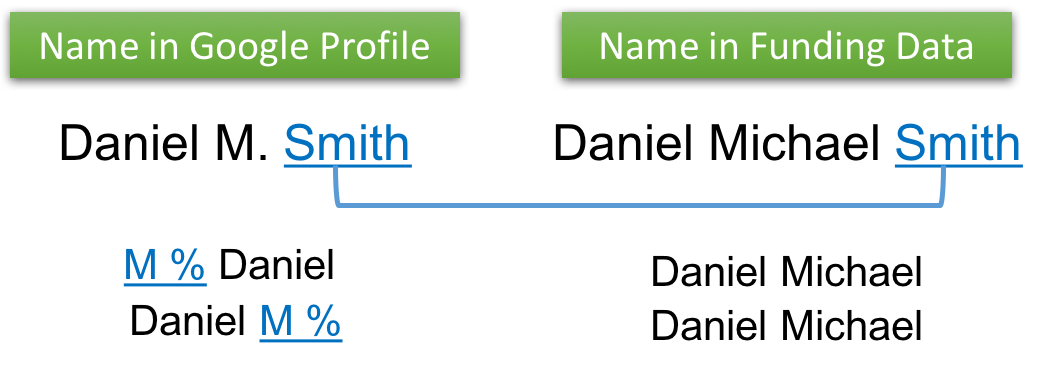
\includegraphics[width=.9\textwidth]{figures/fig-name-dis-example2}
\caption{Example of matching the name in Google Profile with the name in funding data. Daniel M. Smith is considered as Daniel Michael Smith and Daniel Smith.}
\label{alg-example}
\end{center}
\end{figure}




% --------------------------
%\subsection{Within and across profile author name disambiguation}
%% --------------------------
%
%Let $i$ be an index for the Google scholar profile researchers. Within each collaboration profile of $i$,  there are a set of $K_{0}$ raw name strings that you have extracted,  $Names_{k}$ indexed by $k_{i}$. We will use the fact that these strings are associated with profile $i$ in the process of name disambiguation across Google Scholar profiles. The following provides an outline of this procedure: \\
%
%
%A) {\bf Clean last names:}
%Remove strings at end of all $Names_{k}$ that are not last names, and which may not consistently be listed for $k$, e.g. ``Jr.'', ``III'' etc. Hence, each name string  $Name_{k}$ consists ideally of a First name string $FN_{k}$, a Last name string $LN_{k}$, and possibly a Middle name string $MN_{k}$. \\
%
%B)  {\bf Clean middle initial strings within each profile $i$:}  Within each $i$, search for inconsistencies in the use of $MN_{k}$. That is, possibly sometimes the author $k$ is listed as {\it Alexander M Petersen}, sometimes {\it Alexander Petersen}, and sometimes {\it Alexander Michael Petersen}. In this example the Last name string $LN_{k} = Petersen$ and the First name string $FN_{k} = Alexander$ are clearly consistent. But the Middle name string \{$\_$ , M, Michael\} causes some ambiguity if simple string comparison is used,  where $\_$ is a whitespace.
%
%%Hence, for each distinct  surname $FN_{k}$ and last name $LN_{k}$, map all $MN_{k}$ strings to the simplest representation $\hat X$ of just the middle name initials.\\
%
%Then check to see how many different types of {\it Alexander} $\hat X$ {\it Petersen} occur within each $k$, where $\hat X$ is refers to the middle name. Use the following rules for when there are 2 or more types of $\hat W \hat X Petersen$.
%
% \begin{itemize}
% \item If there are only two  types of $Alexander \hat X Petersen$, with $\hat X=$ $\_$ or $M$, then map all of the $Alexander \hat X Petersen$ to $Alexander M Petersen$ for this $i$
% \item If there are only three types of $Alexander \hat X Petersen$, with $\hat X=$ starting with the same initial, $M\_$ or $M$, then map all of the $A\hat X Petersen$ to $Alexander Michael Petersen$ for this $i$
% \item If there are two or more types of $Alexander \hat X Petersen$, say $\hat X=O$ and $\hat X=P$, then keep these $X$ as they are.
%
%%  \item However, if one of those types are a whitespace,  say $\hat X=O$ and $\hat X=P$  and $X= \_$, then we cannot know if the latter possibly corresponds to $O$ or $P$. This case shouldn't occur often. So we can use the simple heuristic that if there is any paper with $AO$ and $A$, then in this case the latter is actually $AP$, and so all $A\_$ are mapped to $AP$. If there are no papers that make obvious this distinction,  then compare the coauthors of $AO$ and $AP$  and $A \_$ within the profile of $i$. Map $A \_$ to $AP$ if they share more coauthors or map $A \_$ to $AP$ if they share more coauthors using the Jaccard Similarity measure to compare.
%\end{itemize}
%
%C)  {\bf Disambiguate coauthors $k$ across the Google Scholar profiles (connecting $i$):} Let  $k$ and $k'$ be coauthors in profiles $i$ and $i'$, respectively.   In this step we would like to identify $k$ and $k'$ that are likely the same person, $k=k'$, allowing us to connect the two profiles $i$ and $i'$ within the coauthor network.\\
%
% If $k$ and $k'$ have the same initials and same surname, then there is a possibility that they are the same individual. Also, if their full first name strings match, this is clearly very positive evidence of this. Let $A_{k,j}$ be the entire combination of First Name and Middle initial $FM_{k,j}$ with the surname $L_{k,j}$ (e.g. {\it Adam B Smith}, or {\it Adam \_ Johnson}) of the coauthor $j$ of the coauthor $k$.
%
% \begin{itemize}
% \item If the full first name strings and the full last name strings are the same, $FN_{k,j}$=$FN_{k',j}$ and $LN_{k,j} = LN_{k',j}$ (e.g. Adam J. Johnson and Adam Johnson), and they both have at least one coauthors in common,  then they are considered the same coauthor.
% \item If we don't have the added information of their full first names then we must rely more heavily on the information from their coauthors. If the first and last names are the same, $FM_{k,j}=FM_{k',j}$ and $LM_{k,j}=LM_{k',j}$, and there are more than 2 middle names with one of the middle name being empty, we do the following -
%
% We compute the number of coauthors in common of the empty middle name author with non-empty middle name authors by comparing the sets of coauthors, $\{j\}$.% and $\{j'\}$.
%
% We assign the empty middle name to that middle name for which there are more number of co-authors in common.
%
% \item If the first name of the author has a hyphen, we check for any other author having the same last name and the first name as the first word of the hyphenated word and middle name starting with the first letter of the second part of the hyphenated word. If any such pair of authors have at least one author in common, we update the first and middle name of the author with the hyphenated middle name to first name and middle name of the matched author.
%
%
%\item If the first name of the author has only two letters, we check for any other author having the same last name and the first name starting with the first letter of the first name and middle name starting with the second letter of the first name. If any such pair of authors have at least one author in common, we update the first and middle names of the author with two letters to first and middle names of the matched author.
%
%\end{itemize}
%Google Scholar data has to be cleaned because it contains many non-english characters. We use regular expression to remove the invalid special characters and translate phonetic characters to english alphabets. We designed and implemented Algorithm \ref{alg:name} to match the author names in Google Scholar with those in NSF/NIH/NASA data. This process helps to improve the quality of results.


